\documentclass[12pt]{article}

\usepackage{amsmath}
\usepackage{graphicx}
\usepackage[numbers]{natbib}
\usepackage{titling}
\usepackage{float}
\usepackage[hidelinks]{hyperref}
\usepackage{amsthm}
\usepackage{listings}
\usepackage{xcolor}
\usepackage{algorithm}
\usepackage{algpseudocodex}
\usepackage{enumitem}


\lstdefinelanguage{glsl}{
    keywords = {if, else, continue, break, for, mat4, vec4, vec3, vec2, return, true, false, bool, int, float, void, char, sampler2D, struct, discard, in, out, layout, version, uniform},
    keywordstyle = \color{red}\bfseries,
    ndkeywords = {gl_Position, gl_FragColor},
    ndkeywordstyle = \color{blue}\bfseries,
    identifierstyle = \color{black},
    sensitive = true,
    comment = [l]{//},
    morecomment = [s]{/*}{*/},
    commentstyle = \color{grey}\ttfamily,
    stringstyle = \color{green}\ttfamily,
    morestring = [b]",
    morestring = [b]'
}

\lstset{
    breaklines=true,
    basicstyle=\ttfamily\small,
    frame=single
}

\graphicspath{{assets/}}
\bibliographystyle{IEEEtranN}

\newcommand{\wideimage}[2][]{%
  \makebox[\textwidth][c]{\includegraphics[width=1.2\textwidth,#1]{#2}}%
}

\pretitle{%
  \vspace*{-5cm}
  \begin{center}
  
\includegraphics[width=\textwidth]{uniLogo.png}\\
  \vspace*{3cm}
}
\posttitle{\end{center}}

\title
{
    {\Huge Creating and Optimising a Fluid Simulation For Use in Video Games} \\
    \vspace*{1cm}
    {\LARGE BSc Computer Science}
}

\author
{
    \vspace*{0.1cm}\huge Sakir Azimkar \\
    \vspace*{1cm}\huge 200823588 \\
    \large Supervised by: Richard Davison
}

\date{April 2025}

\begin{document}

    \maketitle
    \thispagestyle{empty}

    \newpage
    \pagenumbering{arabic}

    \section*{Abstract}
    This dissertation explores the Navier-Stokes equations, which are used to describe the motion of fluids. It briefly looks at an Eulerian implementation introduced by Jos Stam\cite{stam}, before shifting focus on to Lagrangian methods - specifically Smoothed Particle Hydrodynamics (SPH). Furthermore, this paper describes an implementation of this technique. \\ The main goal of this project is to produce a real-time fluid simulation that can be integrated into a video game, with minimal performance loss. It is an optimisation problem, motivated by an interest in the GPU and shader languages. The final project is a Smoothed Particle Hydrodynamics simulation that can reach 600 frames per second with over thirty-two thousand particles on modern hardware.
    
    \newpage

    \section*{Declaration} ``I declare that this dissertation represents my own work, unless explicitly stated otherwise."

    \newpage

    \section*{Acknowledgements}
    I would like to express my deepest gratitude to my supervisor, Richard Davison, for being reliable and helpful throughout the entire project. I'd also like to thank Gary Ushaw, my ``second" supervisor, who was always encouraging and present at our meetings. Lastly, I'd like to thank my friends and family for supporting me during this time. This dissertation is dedicated to these people.
    
    \newpage
    \tableofcontents
    \newpage
    \listoffigures
    \newpage

    \section{Introduction}
    \label{sec:introduction}
    This section highlights the motivations, aims and objectives of this project. It talks about the overall dissertation structure and compares the differences between this project and the initial proposal.
    
    \subsection{Motivation}
    Fluid dynamics are observed in all aspects of daily life and in research. It is crucial to be able to simulate and understand the behaviour of all fluids, including liquids and gases. There already exists a number of different techniques to achieve this, through utilisation of the Navier-Stokes equations. These methods have been crucial in research and in industry. For example in aerospace, which utilises Computational Fluid Dynamics (CFD) for aerodynamic analysis, aircraft design optimisation and thermal management, to name just a few. As our knowledge of fluids and CFD techniques improve, the global market is expected to increase by nearly triple its current value by 2033\cite{market}. Simulations are also essential for cost reduction, as they reduce the need for physical prototypes, which are significantly more expensive to produce.

    In the gaming industry, realistic fluid dynamics are essential to enhance immersion; being able to interact with the ocean in a beach environment is a lot more engaging than the common use of invisible barriers that prevent interaction with the water in many games. A fantastic example of excellent water physics is \textit{Far Cry 6}\cite{farcry6}, as it looks very realistic and is affected by external forces from objects such as vehicles and people swimming.
    
    However, affordable options for advanced fluid simulation are quite difficult to come by for indie developers, who do not have the same funding as triple A companies like \textit{Ubisoft}. As a result, the motivation for this project is to produce a free, lightweight simulation for all types of fluid (not just water). It will also aim to maintain a high performance, so it may be seamlessly implemented into an existing video game with minimal performance loss. This is essential in the gaming industry as lag and low frame rates hinder the overall gameplay experience.

    \subsection{Aim}
    The aim of this dissertation is to utilise the Navier-Stokes equations and Smoothed Particle Hydrodynamics to produce an accurate fluid simulation. The performance (specifically frame rate) of the simulation will be measured and there will be attempts to optimise it. The resulting code should be a 3D fluid flow video game asset that works for Unity.

    \subsection{Objectives}
    \begin{enumerate}
        \item \textbf{Explore Existing Fluid Simulations} - This dissertation will test and experiment with free and accessible simulations available on the internet. It will compare and identify issues with them from the perspective of a game developer searching for a tool to implement into their own game.
        \item \textbf{Navier-Stokes and SPH} - This dissertation will explain what the Navier-Stokes equations are and describe two ways to utilise them in a fluid simulation.
        \item \textbf{OpenGL and C++/GLFW} - This dissertation will briefly mention a graphics API that was used initially in this project and explain why it was chosen. It will then talk about the issues experienced with this API and why it was not utilised in the final project.
        \item \textbf{Unity and Compute Shaders} - This dissertation will talk about the use of Unity and compute shaders to produce a fluid simulation that runs on the GPU.
        \item \textbf{Frame Rate and Performance Investigations} - Throughout this dissertation, the main focus will be on improving the frame rate of the simulation. It will talk about what methods were used to improve the frame rate, such as reprogramming the simulation in shader languages. The overall goal will be to improve the performance of the simulation.
    \end{enumerate}

    \subsection{Changes}
    In the initial project proposal, it was stated that the simulation would be programmed in \textit{C++}, using \textit{GLFW}\cite{glfw} to create windows and display the graphics created by the graphics API that I would be using, \textit{OpenGL}\cite{opengl}. However, later in development this decision was changed to utilising the \textit{Unity} game engine\cite{unity} and compute shaders. Reasoning will be provided in the What was Done and How section.

    Additionally, the project proposal stated that the simulation would be first created in two dimensions and later upgraded to three. It was decided to skip this step as the development process was mostly the same, the only difference being whether the vectors contained two or three values. This was to save development time and allow more focus on optimisation.

    \subsection{Dissertation Structure}
    
    \subsubsection{Time Structure}
    
    \begin{figure}[H]
        \makebox[\textwidth][c]{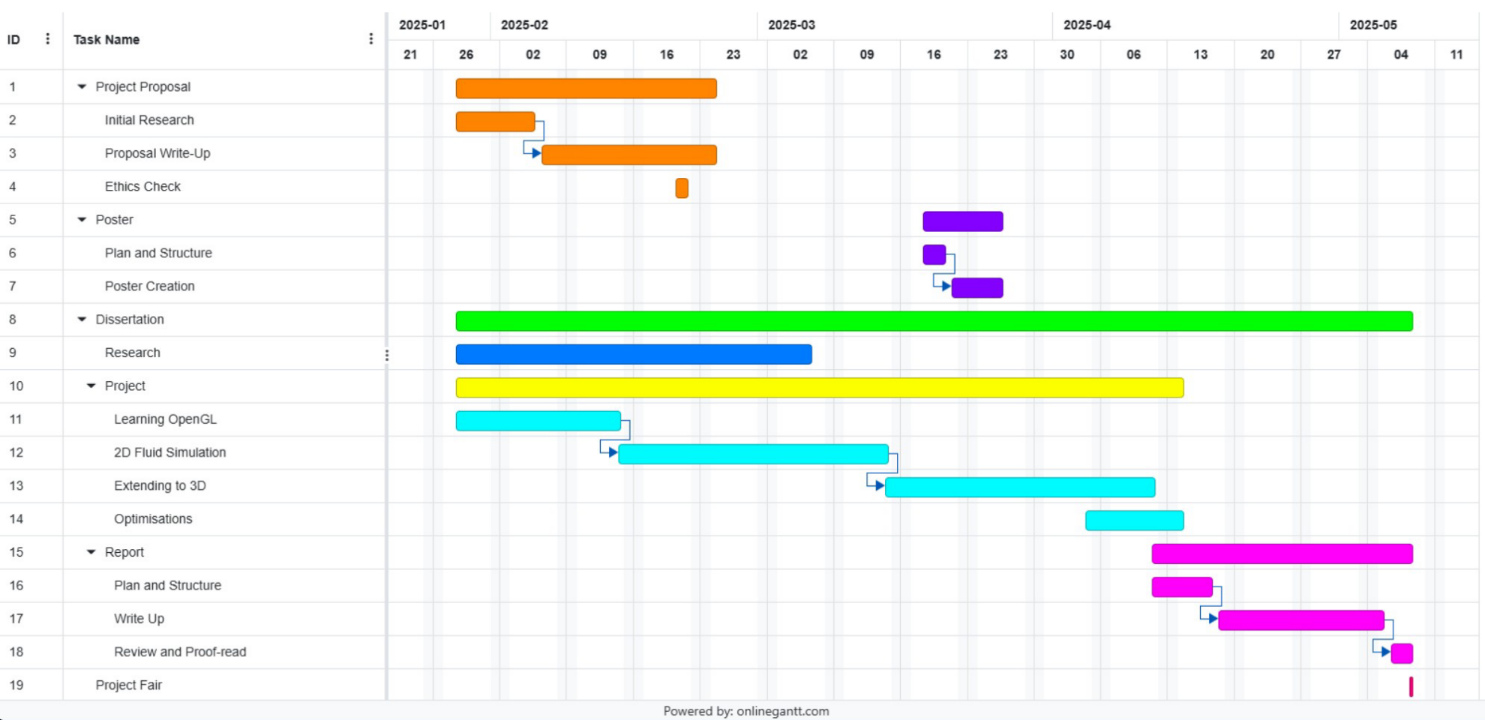
\includegraphics[width=1.4\textwidth]{ganttChart.png}}%
        \caption{Gantt chart of project timeline \cite{onlinegantt}}
    \end{figure}

    \subsubsection{Dissertation Outline}

    \begin{itemize}
        \item \hyperref[sec:introduction]{\textbf{Introduction}} \\
        An introduction to the dissertation, outlining the motivation, aim, objectives and overall project structure. 
        \begin{itemize}
            \item Motivation
            \item Aim
            \item Objectives
            \item Changes
            \item Structure
        \end{itemize}
        \item \hyperref[sec:backgroundreview]{\textbf{Background Review}} \\
        A breakdown of research performed before and during the project.
        \begin{itemize}
            \item Existing fluid simulations
            \item Software Tools
            \item Requirements
        \end{itemize}
        \item \hyperref[sec:whatwasdoneandhow]{\textbf{What was Done and How}} \\
        An explanation of how the simulation was implemented, including the methods learned and processes involved.
        \begin{itemize}
            \item Mathematics and Physics
            \item OpenGL
            \item Unity
            \item Compute Shaders
            \item GPU Instancing
            \item Optimisations
        \end{itemize}
        \item \hyperref[sec:resultsandevaluation]{\textbf{Results and Evaluation}} \\
        A complete analysis of frame rate improvements over the course of the project and results obtained.
        \begin{itemize}
            \item Frame Rate
            \item Simulation Types Produced
            \item Advantages and Disadvantages of Each Implementation
            \item Requirements
        \end{itemize}
        \item \hyperref[sec:conclusion]{\textbf{Conclusion}} \\
        A conclusion that describes fulfilment of objectives, what was learned and future work.
        \begin{itemize}
            \item Aims and Objectives
            \item Achievements
            \item What was Learned
            \item Future Work
        \end{itemize}
    \end{itemize}

    \newpage

    \section{Background Review}
    \label{sec:backgroundreview}
    This section shows the research made on this dissertation. It talks about relevant background resources that were used for different parts of the development process.
    
    \subsection{Strategy}
    There are three main components that needed to be researched at the start of this project:
    \begin{itemize}
        \item Exploring existing fluid simulations
        \item Software Tools
        \item Fluid simulation methods
    \end{itemize}
    \sloppy
    All three of these sections are integral in achieving a functional, lightweight simulation and thus needed to be researched before beginning. Below is an outline of the papers, videos and other resources that were used to understand these topics.

    \subsection{Exploring existing fluid simulations}
    It is important to understand current existing options that are available and describe their benefits and limitations in the context of video games.

    \subsubsection{WebGL Implementations}

    ``WebGL (Web Graphics Library) is a JavaScript API for rendering interactive 2D and 3D graphics within any compatible web browser without the use of plug-ins. WebGL is fully integrated with other web standards, allowing GPU-accelerated usage of physics, image processing, and effects in the HTML canvas".\cite{webglwikipedia}

    There are a lot of fantastic \textit{WebGL} implementations of fluid motion that are easily accessible due to their availability in a web browser. An example is the one developed by PavelDoGreat on GitHub.

    \begin{figure}[H]
        \wideimage[]{webGLGas.png}
        \caption{\textit{WebGL} Fluid Simulation by PavelDoGreat on GitHub \cite{webgl1}}
    \end{figure}

    This simulation showcases a gaseous fluid made up of different, randomly-generated colours. They appear to mostly be for aesthetic purposes. The screen begins completely black and requires the user to input an external force by left-clicking and moving the cursor across the screen. There is a control panel on the top right corner, which allows the user to change various settings, such as density diffusion and vorticity. This is a great visual aid for educational purposes as it allows the user to see the visual impacts that these variables have on the fluid in real time. As an educational tool, this is an excellent visual aid; the immediate feedback and colourful representation make it easy to understand complex fluid dynamics concepts. In the context of video games, however, the colours are a bit unnecessary. This can be easily rectified if someone were to use it in their game, but they would need to make a number of modifications to the existing code to make it independent of user input (for the more common uses of fluids in games).

    Here is another example of a \textit{WebGL}-based fluid simulation available for free online, developed by Grant Kot.

    \begin{figure}[H]
        \wideimage[]{webGLParticles.png}
        \caption{\textit{WebGL} Fluid Simulation by Grant Kot. \cite{webgl2}}
    \end{figure}
    
    This simulation excels in visualising fluid interactions, particularly between liquids of varying masses - represented by four distinct colours. You can use the mouse and different keybinds to manipulate the fluid with a range of forces, such as lifting a portion of it up (as shown in figure 3), or creating dynamic collision objects that follow the cursor. It behaves with realistic motion that is driven by gravity and internal pressure and user interaction is only optional.

    Conversely, there is a performance issue with this project. During testing, the simulation peaked at around 50 frames per second. This is completely fine when exploring the fluid in a web browser or for educational demos, but becomes a much larger issue when using it as a video game asset, as video games prefer to be consistently above 60 frames per second - to maintain responsiveness and overall gameplay fluidity. Further optimisations would be required of this simulation in order to utilise it in a video game environment.

    WebGL simulations, however, work exceptionally in very simple browser games. Here is an example called \textit{Interplanetary Postal Service}\cite{ips}, which was created by Sebastian Macke, for a coding competition with a strict 13KB size limit.

    \begin{figure}[H]
        \wideimage[]{webGLIPS.png}
        \caption{\textit{Interplanetary Postal Service} by Sebastian Macke \cite{ips}}
    \end{figure}

    As the game's core mechanics are very simple (use WASD to power the post lander on to the landing pads), there is very little need for optimisations. This allows it to run consistently at over 60 frames per second. This demonstrates how WebGL-based simulations can deliver high performance and smooth interactivity when used for lightweight, focused experiences - which most video games aren't.

    While all of these examples are incredibly impressive, they would not function well in more complicated, non-web-based video games. The first two are built as standalone browser-based visualisations for the purposes of aesthetics and education. Although all of these can be rewritten and ported to OpenGL-based games, there is a lot of upfront work required to do so; they do not work out-of-the-box. They are also only two-dimensional, which means further modifications would be required necessary to adapt them for 3D environments. Furthermore, for games written using pre-existing game engines such as Unity, most of the existing JavaScript simulation code would have to be rewritten into a language that is compatible with the engine, such as \textit{C\#}. One of the aims of this dissertation is to produce a 3D asset that is ready to use in Unity without requiring extensive modifications.

    \subsubsection{Unity Assets}

    There are a few choices on the \textit{Unity Asset Store}\cite{unityasset}. However, there are a few issues with each of the available options.

    \begin{figure}[H]
        \wideimage[]{obiFluid.png}
        \caption{\textit{Obi Fluid}, Unity Asset \cite{obi}}
    \end{figure}

    The most popular option appears to be \textit{Obi Fluid}, which advertises ``multi-threaded AAA quality fluid simulations" on its store page. From the screenshots and videos provided, this does appear to be the case. However, with its steep price tag, it is difficult to verify as many developers are understandably hesistant to spend over £40 on a single asset. Additionally, the store page mentions that the simulation may have performance issues in larger projects and should only be used for smaller scale projects or 2D game simulations, making it an unfit choice for 3D games or large bodies of fluid.

    \begin{figure}[H]
        \wideimage[]{KWS.png}
        \caption{\textit{KWS Water System Standard} \cite{kws}}
    \end{figure}

    Another fantastic asset is the \textit{KWS Water System}. It has a lot of incredibly useful features, such as refraction, volumetric lighting and screen space reflections. Furthermore, it has optimisations implemented such as instanced rendering and view culling, so it is possible to simulate much larger bodies of fluid with minimal performance issues. This would be an outstanding asset for video games, if it weren't for the even steeper price tag of over £60.

    In addition to these examples, there are many available assets that don't simulate actual fluid motion or behavior, but instead create the illusion of it by only simulating the surface. This is a suitable option for games that don't require fluid interaction, but that falls outside the scope of this dissertation. One of the main motivations of this project is that the simulation is accessible to all kinds of developers, so it will be free unlike these examples.
    
    \subsubsection{Fluids in Video Games}

    It is also important to understand the fluid simulations that are actively present in existing video games. There aren't many games allow the player to interact with the water physically, due to the high performance cost required to implement these features.

    \begin{figure}[H]
        \wideimage[]{fromDust.png}
        \caption{\textit{From Dust} Gameplay \cite{fromdustvideo}}
    \end{figure}

    \textit{From Dust}\cite{fromdust} is a god game where the player manipulates matter such as lava, soil and water. In the gameplay video\cite{fromdustvideo}, it is clear that the sand when placed and moved around displaces the water realistically. While the visual quality of the static sea surface may appear simplistic by modern standards, the game's real-time manipulation of large quantities of matter was groundbreaking for its era over thirteen years ago. Albeit impressive visually, there was a lot of computational resources required to run such a large scale simulation. As a result, there was quite a few complaints about the game being capped at 30 frames per second\cite{dsog}, which was very low even back then.
    
    \begin{figure}[H]
        \wideimage[]{clairObscur.png}
        \caption{A screenshot of water blocked by an invisible wall in Clair Obscur: Expedition 33}
    \end{figure}

    Even nowadays there are a lot of video games that don't utilise realistic fluid flows because of their high computational resource requirement. An example of this is a game that released just this month, \textit{Clair Obscur: Expedition 33}\cite{clairobscur}.
    While the simulation is visually stunning, it is not possible to interact with the water. There is a loss of immersion here, especially considering the position of this water. It is located at the end of the prologue, after the character has left the island they have resided on their entire life to explore the abandoned mainland. The character, having never before set foot beyond their home, should be experiencing a profound sense of unfamiliarity due to a heavy environment change. The static and artificial appearance of the river diminishes this intended narrative impact, disconnecting the character from the player.

    \begin{figure}[H]
        \wideimage[]{farCry6.png}
        \caption{Helicopter physics in Far Cry 6 \cite{farcry6video}}
    \end{figure}

    A modern game that does an excellent job at fluid simulation is \textit{Far Cry 6}. As shown in Figure 9, the wind produced by the helicopter's turbines visibly pushes the water away from the vehicle. Furthermore, the player is able to swim and dive into the fluid, as well as observe external forces acting upon it when objects, such as explosives, are thrown into the water. This would be an ideal fluid simulation approach for many games seeking realistic water interactions. However there are a few issues with this. Since \textit{Far Cry 6} is a proprietary, AAA game, its source code is not visible to the public, as thus the simulation is not accessible by anyone else.
    
    Since the release of this game, the former water lead tech, Zhenyu Mao, has moved on to other projects with \textit{Lightspeed Studios}, and has developed a new water rendering solution for games. In an interview\cite{zhenyu}, Mao mentions ``Thanks to Dr. Wu's expertise, we have developed a proprietary solution that generates natural water flow that interacts harmoniously with the environment. Our water simulation can generate accurate flow around objects, creating realistic turbulence and generating foam in the appropriate places." This sounds incredibly promising, but is currently still a proprietary, in-house solutiona available to \textit{Lightspeed Studios} only. There is a presentation available online about the physics behind this solution\cite{zhenyupresent}, but that is not in the scope of this dissertation.

    \subsubsection{Conclusion}

    While there are a lot of fluid simulations available online, few are practical for use within 3D video games; they are often computationally taxing and thus would not be a feasible asset to utilise without significant prior optimisation and modifications. The options that do satisfy these conditions are usually proprietary and restricted to the studio it was developed in - or come at a premium cost inaccessible to some developers. Therefore, the motivation for this dissertation is to develop a freely accessible, efficient 3D fluid simulation that can be integrated into modern video games without significant performance trade-offs.

    \subsection{Software Tools}

    Choosing the correct set of tools is essential for an optimisation problem. They must be lightweight in nature and avoid unnecessary overhead in order to achieve the best performance possible.

    \subsubsection{Graphics API vs. Existing Game Engine}

    \begin{figure}[H]
        \wideimage[]{unityInterface.png}
        \caption{Empty Unity\cite{unity} scene}
    \end{figure}

    Game engines have the advantage of simplicity, leading to a faster development cycle. There are a lot of available pre-built tools, editors and assets that allow rapid prototyping and game development. For the purposes of this dissertation, many of these tools are not necessary. For instance, the physics engine will not be utilised as all physics will be manually coded. However, many of these tools would be beneficial for this project. For example, all linear algebra calculations related to camera depth and appearance have already been implemented. This means that by simply loading a model into the scene, it will automatically be rendered in 3D with realistic lighting. This saves the hassle of writing it all from scratch if a grpahics API were to be implemented.

    Game engines also benefit from large, active communities. There are plenty of tutorials, forums and online resources created by other developers. This makes it easier to find solutions to common problems, whether they involve problem solving or bug fixing. Graphics APIs are not as commonly utilised due to their increased complexity and thus have fewer resources available. However, there are two great tutorials for both \textit{OpenGL} and \textit{Vulkan}\cite{vulkan} that fully explain and provide an implementation for the setup of the graphics rendering pipeline \cite{learnopengl}\cite{vulkantutorial}.

    Graphics APIs have the added benefit of greater control and customisation due to their lack of abstration and increased level of understanding required. Every phase in the graphics rendering pipeline can be controlled manually, giving the developer more freedom and flexibility. There is also no overhead from the game engine, which may also slightly improve performance. Furthermore, once a project is begun within an engine, it is bound by its licenses, giving the developer less freedom.

    Due to an enthusiasm to learn more about the graphics rendering pipeline and more low-level graphics interactions, it was decided at this point that a graphics API would be utilised over a game engine. Aforementioned in the project proposal, this was with the caveat that a swap to a game engine (specifically \textit{Unity}, due to prior experience) would occur if insufficient progress was made in the strict timeframe of this project. Considering the changes made to this dissertation in comparison to the project proposal, it is clear that this alteration was eventually realised.

    \subsubsection{OpenGL vs. Vulkan}

    As a graphics API was decided, the next choice was between \textit{OpenGL} and \textit{Vulkan}. \textit{DirectX} was not considered due to its lack of cross-platform compatability, as it was specifically designed for \textit{Windows} and \textit{XBox}. This was a relatively simple decision, as \textit{OpenGL} is considered the beginner option, and \textit{Vulkan} is not recommended for new graphics programmers by Alexander Overvoorde, the writer of \textit{Vulkan Tutorial}: ``Vulkan is targeted at experienced graphics programmers. You should start with an easier language than \textit{C++} and an easier API than Vulkan'' \cite{vulkancomment}. Although \textit{Vulkan} is a better choice for future-proofing (as \textit{OpenGL} is no longer receiving updates), this reasoning was not significant justification; the project can be rewritten in the future with more time and experience. Thus, \textit{OpenGL} was selected, accompanied by the \textit{C++} language due to previous experience with the language.
    
    \subsection{Fluid Simulation methods}

    This section talks about two simulation methods involving the Navier-Stokes equations.

    \subsubsection{Navier-Stokes Equations}

    \begin{equation}
        \frac{\partial{\textbf{u}}}{\partial{t}} + (\textbf{u} \cdot\nabla)\textbf{u} = v\nabla^2 \textbf{u} - \frac{1}{\rho}\nabla p + \textbf{f}
    \end{equation}

    Equation 1 is a non-linear partial differential equation that describes fluid motion\cite{slides}. The first term, $\frac{\partial{\textbf{u}}}{\partial{t}}$, represents the change in velocity over time at a fixed point, where $\textbf{u}$ is the velocity field of the fluid. $-(\textbf{u}\cdot\nabla)\textbf{u}$ is called the advection term. Advection is described as ``the transport of a substance or of heat by the flow of a liquid"\cite{cambridge}. In fluid dynamics, this may also refer to the transport of a property due to fluid flow. $\nabla$ is a vector of partial derivatives: $\nabla = (\frac{\partial}{\partial x}, \frac{\partial}{\partial y}, \frac{\partial}{\partial z})$. Taking the dot product of \textbf{u}, a vector, and this operator, $\textbf{u}\cdot\nabla$, gives us a directional derivative - it describes the direction that a property is changing.

    \begin{equation*}
        (\textbf{u}\cdot\nabla)\textbf{u} \equiv u_x \frac{\partial \textbf{u}}{\partial x} + u_y \frac{\partial \textbf{u}}{\partial y} + u_z \frac{\partial \textbf{u}}{\partial z}
    \end{equation*}

    This term thus describes the advection of velocity, which is also referred to as convective acceleration, ``the effect of acceleration of a flow with respect to space''\cite{nswikipedia}.

    There are three more terms on the right hand side of the equation: the diffusion/viscosity term, pressure and external forces. Sometimes written as $\nabla \cdot (v\nabla\textbf{u})$, the viscosity term describes how the fluid motion is damped due to its viscosity. Fluids with a higher viscosity constant $v$ tend to have stronger resistance, resulting in stronger smoothing and slower flows. $\nabla^2$ is also known as the Laplacian operator. The Laplacian is obtained by summing the second partial derivative with respect to each variable component-wise:

    \begin{equation*}
        \nabla^2\textbf{u} \equiv (\frac{\partial^2{u_x}}{\partial{x^2}} + \frac{\partial^2{u_x}}{\partial{y^2}} + \frac{\partial^2{u_x}}{\partial{z^2}}, \frac{\partial^2{u_y}}{\partial{x^2}} + \frac{\partial^2{u_y}}{\partial{y^2}} + \frac{\partial^2{u_y}}{\partial{z^2}}, \frac{\partial^2{u_z}}{\partial{x^2}} + \frac{\partial^2{u_z}}{\partial{y^2}} + \frac{\partial^2{u_z}}{\partial{z^2}})
    \end{equation*}

    Multiplying this value by a viscosity constant determines how much the velocity is smoothed or evened-out by viscous forces. If the Laplacian is positive, it means that the velocity is lower at that point than its neighbours, so a larger positive force is applied; a negative Laplacian applies force in the opposite direction.

    Pressure is simply defined as ``the amount of force acting on a certain area"\cite{bbcbitesize}, or force acting per unit area. As a result, a pressure gradient produces a force that pushes the fluid from areas of high pressure to areas of low pressure. This is described by the second term, $-\frac{1}{\rho}\nabla{p}$, where $\nabla{p}$ is the pressure gradient, and $\rho$ is the density of the fluid at this position. Since gradients point in the increasing direction, the negative is taken so the fluid moves away from the direction of increasing pressure. Additionally, this gradient value gives force acting per unit volume, but the previous terms have been accelerations. This is corrected using Newton's Second Law, $F = ma$. Since density is the mass per unit volume of the fluid, the pressure gradient is multiplied by the reciprocal of the density to obtain the acceleration. Below is a correction of the SI units to obtain acceleration.

    \begin{proof}
        $$\left[\nabla{p}\right] = \frac{N}{m^3} = \frac{kg \cdot ms^{-2}}{m^3} = \frac{kg}{m^2\cdot s^2}$$
        $$\left[\rho\right] = \frac{kg}{m^3}$$
        $$\frac{\left[\nabla{p}\right]}{\left[\rho\right]} = \frac{kg}{m^2 \cdot s^2} \cdot \frac{m^3}{kg} = \frac{m}{s^2}$$
    \end{proof}
    
    The final term accounts for external forces that act on the fluid, such as gravity. These forces are included to correctly describe changes in momentum according to Newton's Second Law.

    \begin{equation}
        \frac{\partial{\rho}}{\partial{t}} = -(\textbf{u}\cdot\nabla)\rho + \kappa\nabla^2 \rho + S
    \end{equation}

    Equation 2 has very similar structure to Equation 1, however this one is used in the calculation of a scalar quantity, density. As a result, there is no pressure force term, and external forces is replaced by an external source term S, which adds or removes density from the system. The viscosity constant is also replaced with $\kappa$, the diffusion constant. This measures how fast the property (in this case density) diffuses through the fluid.

    \subsubsection{Eulerian Implementations}

    Eulerian, or grid-based implementations for fluid dynamics treat the fluid as a grid of cells.
    
    \begin{figure}[H]
        \begin{center}
            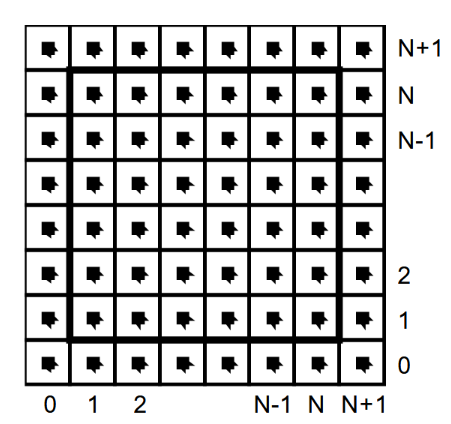
\includegraphics{gridFluid.png}
            \caption{Computational grid with densities and velocities defined in their centres \cite{stam}}
        \end{center}   
    \end{figure}

    Figure 11 is a computational grid of cells by Jos Stam. There is an extra layer of cells around the grid to account for boundary conditions. This method utilises Equation 2 to produce a density diffusion solver, where each cell either adds or removes density from its neighbours. Due to distance of other cells, there is no need to include any others in this calculation, as their impact will be negligible and slow the simulation down quite considerably.

    \begin{figure}[H]
        \begin{center}
            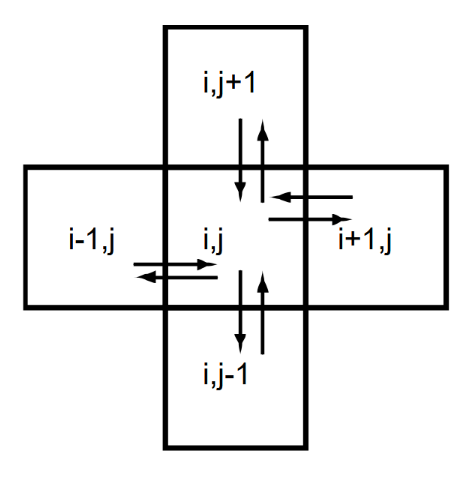
\includegraphics{neighbourDiff.png}
            \caption{Density exchange through diffusion between neighbours \cite{stam}}
        \end{center}   
    \end{figure}

    After this diffusion has occured, the centres of the grids are treated as sample points traced through the velocity field, similar to Lagrangian methods. In order to convert the ``particles" back into grid cells, there are two grids used: a grid of cells containing the old density values and a second grid containing the new density values. The new positions are traced backwards through the velocity field to find the original grid cell, and assign this value to the new position.

    Finally, there is the projection step, which ensures that the updated velocity fields are mass conserving, by enforcing the incompressibility condition: 
    
    \begin{equation}
        \nabla \cdot \textbf{u} = 0
    \end{equation}
    
    In order to perform this step, the divergence of the velocity field is computed and a Poisson equation is solved for some pressure-like field $p$
    
    \begin{equation}
        \nabla^2{p} = \nabla \cdot \textbf{u}
    \end{equation} 
    
    This is then utilised to project the velocity on to a divergence-free value
    
    \begin{equation}
        \textbf{u}_{new} = \textbf{u} - \nabla{p}
    \end{equation}

    \begin{figure}[H]
        \begin{center}
            \wideimage[width=0.7\textwidth]{eulerianEG.png}
            \caption{Eulerian simulation \cite{eulerianeg}}
        \end{center}
    \end{figure}

    There are many different methods to achieve fluid flow with Eulerian implementations, but more detail is out of the scope of this dissertation.

    \subsubsection{Lagrangian Implementations}

    Lagrangian implementations of fluid flow involve treating the fluid as small parcels or particles of fluid. These particles influence their neighbours but are not confined to grid cells. As a result, more calculations are required in determining which particles are within effective range. A classic example of a Lagrangian method is Smoothed Particle Hydrodynamics (SPH).

    SPH was initially developed by Gingold, Monaghan and Lucy in 1977 for the purposes of astrophysics\cite{sca}. Since the particles are independent nodes, this method is meshfree, which improves parallelisation. Considering the expensive computations required, parallelisation is fundamental in improving performance. Furthermore, conservation of mass is guaranteed; the particles represent mass and the particles do not disappear at any stage of the simulation.

    Furthermore, this method utilises the Navier-Stokes equations to produce the following generalised SPH equation:

    \begin{equation}
        A_S(\textbf{r}) = \sum_{j}{m_j \frac{A_j}{\rho_j}W(\textbf{r} - \textbf{r}_j, h)}
    \end{equation}

    For each particle with position $\textbf{r}$, every other particle $j$ with mass $m_j$, density $\rho_j$, position $\textbf{r}_j$ and property $A_j$ is iterated through to calculate that particle's total property quantity. $W(r, h)$ is a smoothing kernel that is defined differently for each property, where $r$ is the distance between the two points $\lvert\textbf{r} - \textbf{r}_j\rvert$ and $h$ is the smoothing radius for each particle. After a large enough distance $r > h$, the value of the smoothing kernel becomes 0; the particle is too far away to provide any significant influence. As a result, this calculation only needs to be performed on particles that are close enough, a key optimisation step for this method. Further details regarding this method can be found in the \hyperref[sec:whatwasdoneandhow]{"What Was Done and How"} section of this dissertation.

    \subsubsection{Chosen Implementation}

    Due to the simpler parallelisation and streamlined process of meshfree methods, this dissertation will focus on the implementation and optimisation of a Lagrangian fluid simulation, specifically utilising Smoothed Particle Hydrodynamics.

    \newpage

    \subsection{Requirements}

    Using the background research, a set of functional and non-functional requirements may be produced.

    \subsubsection{Functional Requirements}

    \begin{enumerate}[label=\textbf{F.R. \arabic*}]
        \item The fluid will be rendered with particles that represent parcels of fluid.
        \item The simulation will accurately model fluid behaviour, including properties such as viscosity, density and pressure.
        \item The fluid will be affected by gravitational forces.
        \item The fluid will remain within a box, which has adjustable dimensions.
        \item The user can manipulate the fluid by dragging an object through it.
    \end{enumerate}

    \subsubsection{Non-Functional Requirements}

    \begin{enumerate}[label=\textbf{N.F.R. \arabic*}]
        \item The simulation will run at a high frame rate to ensure smooth gameplay.
        \item There will be attempts to reduce the overall memory consumption of the simulation.
        \item The simulation will be stable with minimal bugs or crashes.
        \item The simulation will remain stable and flow accurately with no stuttering or jumping.
        \item The simulation will run in real time, with adjustable properties that also update in real time.
        \item The simulation will be modular; new fluid types and behaviours can be added in the future with ease.
    \end{enumerate}

    \newpage

    \section{What Was Done and How}
    \label{sec:whatwasdoneandhow}

    This section talks about everything learned and implemented throughout the development process.

    \subsection{Software Development Model}

    This project adopts the agile development model. There are four core values of this method\cite{geekagile}:
    
    \begin{itemize}
        \item Individuals and Interactions over Processes and Tools
        \item Working Software over Comprehensive Documentation
        \item Customer Collaboration over Contract Negotiation
        \item Responding to Change over Following a Plan
    \end{itemize}

    While not all of these principles are directly applicable in this context, the emphasis on adaptability remains essential. Regular weekly meetings with the project supervisor supports an iterative approach and allows the scope to shift due to time constraints or technical challenges. For example, the graphics rendering method was switched from \textit{OpenGL} to \textit{Unity} in order to guarantee completion within the given timeframe. Additionally, as the primary goal of this dissertation is optimisation, extensive documentation is unnecessary; the simulation only needs to be demonstable and functional. Development was carried out in short iterations, with weekly goals set and versioned using \textit{Git}.

    \subsection{Graphics Rendering Pipeline}

    In order to utilise the \textit{OpenGL} graphics library\cite{opengl}, it is important to first understand the API and the graphics rendering pipeline. This was achieved with the tutorials provided by the\textit{Learn OpenGL} website created by Joey de Vries\cite{learnopengl} as well as resources provided by the project supervisor.

    The graphics pipeline takes a set of 3D coordinates as an input and transforms them into coloured 2D pixels that are displayed on the screen. Developers interact with this pipeline through the use of shaders, which are programs executed in parallel on the GPU.

    \begin{figure}[H]
        \wideimage[]{graphicsPipeline.png}
        \caption{Graphics Rendering Pipeline \cite{learnopengl}}
    \end{figure}

    \subsubsection{Vertex Shader}

    Vertex shaders process vertices and calculates their coordinates in clip space. This tells the computer if the vertex is in camera view or if it should be discarded \cite{shadertutorial}. They can be used to perform calculations on models, such as rotations and translations. They utilise uniform matrices, usually called model, view and projection that are passed to the shader from the main program.

    \paragraph{Model}matrices are used to represent the centre of the model being drawn by the shader, which has been transformed into the necessary position in the world. Multiplying a vertex by this value describes where the vertex exists relative to the centre of the model.

    \paragraph{View}matrices describe the camera's position and multiplying this matrix with the vertex's world position ($model \cdot vertex$) determines the vertex's position relative to the camera.

    \paragraph{Projection}matrices describe the perspective of the camera, including variables such as fov and aspect ratio. These values can distort and scale the appearance of the model and thus need to be considered. Multiplying this matrix with the resultant calculation of the other matrices will achieve this.

    An example of a very basic \textit{OpenGL} vertex shader is shown below.

    \begin{lstlisting}[language=glsl]
        #version 330 core

        layout (location = 0) in vec3 position;

        uniform mat4 model;
        uniform mat4 view;
        uniform mat4 projection;

        void main()
        {
            gl_Position = projection * view * model * vec4(position, 1.0);
        }
        
    \end{lstlisting}

    \subsubsection{Geometry Shader}

    This optional shader takes a collection of vertices that form a primitive, and uses them to form other shapes. An example of this may involve producing a new vertex position that splits a triangle in half to form two smaller triangles. This step is not utilised in this project.

    \subsubsection{Shape Assembly}

    Shape assembly, or primitive assembly, uses the data from either the vertex or geometry (if used) shader to draw the primitive defined, usually a triangle.

    \subsubsection{Rasterization}

    Rasterization involves mapping the resulting primitives to the corresponding pixels on the final screen, producing fragments. A fragment is all the data required for the API to render a single pixel. Then, all fragments not within the camera view are discarded.

    \subsubsection{Fragment Shader}

    The fragment shader is used to determine the final colour of the pixels. Since only the vertices of the primitives are given, interpolation is used to calculate the colour of the pixels in between the vertices. This is done automatically by the graphics API by checking its position and distance relative to all of the primitive's vertices and determines the colour based off this value. For example, setting each vertex of a triangle primitive to a different primary light colour (red, green, blue), produces the following result:

    \begin{figure}[H]
        \begin{center}
            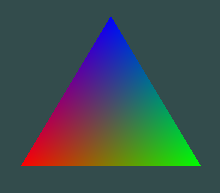
\includegraphics{rainbowTriangle.png}
            \caption{Rainbow Triangle rendered with OpenGL}
        \end{center}
    \end{figure}

    This is done by passing the desired RGBA values of the vertices through to the vertex shader, which then passes the data through the pipeline to the fragment shader.

    \subsubsection{Tests and Blending}

    The final stage of the pipeline involves setting the opacity, or alpha of the pixels and adjusting/blending their colours appropriately. Also, if any models are overlapping, the colours of the model at the back are discarded as they should appear covered by the front model.

    \subsection{GLFW and GLAD}

    Creating an \textit{OpenGL} context and a window to draw the graphics in are OS-specific operations. As a result, an external library is required. \textit{GLFW}\cite{glfw} is a library written in C that does all of this. Additionally, \textit{OpenGL} is a specification. It is up to the manufacturer of the graphics card to implement the specification to a driver compatible with the card. As a result, the specific location of \textit{OpenGL} functions are not consistent and need to be retrieved manually. \textit{GLAD}\cite{glad} is a library that does this automatically.

    \subsection{Learn OpenGL}

    Using this knowledge of the rendering pipeline, the \textit{OpenGL} specification and the \textit{Learn OpenGL} website, it is now possible to render particles on to the screen and apply transformations to them. See the \hyperref[sec:appendices]{appendices} for code snippets and graphics produced from this tutorial. 
    
    \begin{figure}[H]
        \begin{center}
            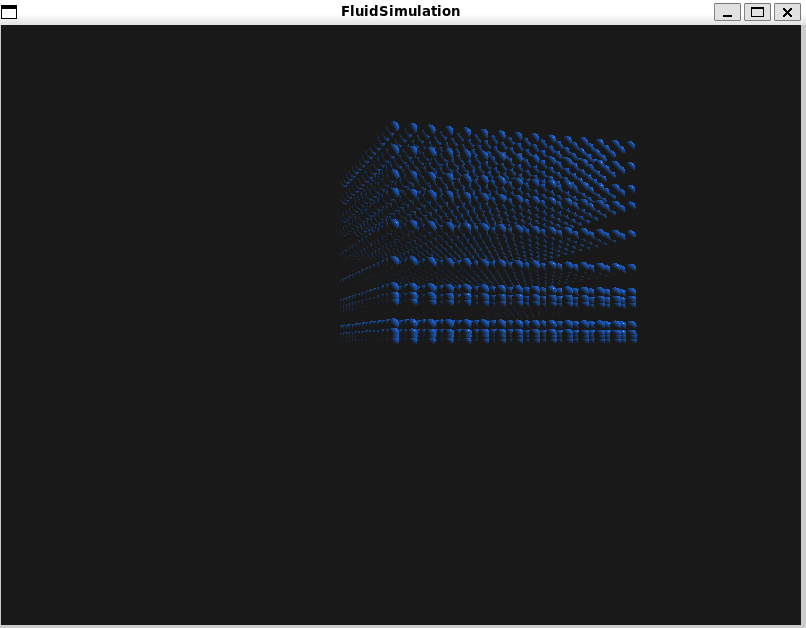
\includegraphics[width=0.9\textwidth]{openGLProg.png}
            \caption{Final progress with OpenGL}
        \end{center}
    \end{figure}
    
    Learning the theory behind the graphics rendering pipeline and OpenGL took longer than anticipated. It was at this point that the decision to swap to Unity was made. Figure 16 displays the final progress achieved with \textit{OpenGL} and \textit{C++}. In the simulation, 1000 particles are rendered in a grid-like structure. They move downwards as a result of a gravitational force and bounce off the ``floor" ($y = 0$) with slight damping. There are currently no forces calculated between the particles and as a result they move through each other.

    \subsection{Simulation Loop}

    This section provides the theory and pseudocode for the update loop of this simulation. Undefined variables that appear in the pseudocode are assumed to be defined constants outside the simulation loop. The following implementation is presented in the paper ``Particle-Based Fluid Simulation for Interactive Applications'', by Matthias Müller, David Charypar and Markus Gross\cite{sca}.

    \begin{algorithm}
        \caption{Simulation Loop}

        \begin{algorithmic}[1]
            \ForAll{particles $i$}
                \State calculate density and pressure
            \EndFor

            \ForAll{particles $i$}
                \State compute forces
            \EndFor

            \ForAll{particles $i$}
                \State update velocity and position
                \State resolve collisions
            \EndFor
        \end{algorithmic}

    \end{algorithm}

    \subsubsection{Density and Pressure}

    Using the aforementioned generalised SPH equation, it is possible to compute the density of each particle by replacing $A$ with $\rho$. Furthermore, in this simulation each particle will be the same size and mass $m$.

    \begin{equation}
        \rho_S(\textbf{r}) = \sum_{j}{m_j \frac{\rho_j}{\rho_j}W(\textbf{r} - \textbf{r}_j, h)} \equiv m\sum_{j}{W(\textbf{r} - \textbf{r}_j, h)}
    \end{equation}

    The chosen smoothing kernel for density is the Poly6 kernel described in the paper above\cite{sca}. This kernel is defined as:

    \begin{equation}
        W_{poly6}(\textbf{r}, h) = \frac{315}{64\pi{h}^9}
        \begin{cases}
            (h^2 - r^2)^3 & \text{if } 0 \leq r \leq h \\
            0 & \text{otherwise}
        \end{cases}
    \end{equation}

    For the purposes of speed, we use a modified version of the ideal gas equation to calculate pressure

    \begin{equation}
        p = k(\rho - \rho_0)
    \end{equation}

    where $k$ is a unique gas constant for the fluid and $\rho_0$ is the fluid's resting density.

    The pseudocode for this calculation programatically is as follows

    \begin{algorithm}[H]
        \caption{\textsc{CalculateDensity}(Particle $p$)}
    
        \begin{algorithmic}[1]
            \State total $=$ 0
            
            \ForAll{particles $i$}
                \State distance $=$ \textsc{magnitude}($p$.position - $i$.position)

                \If{distance $\leq$ smoothingRadius}
                    \State total $+=$ \textsc{poly6}(distance)
                \EndIf
            \EndFor

            \State $p$.density $=$ particleMass $\cdot$ total
            \State $p$.pressure $=$ gasConstant $*$ ($p$.density $-$ restDensity)
        \end{algorithmic}

    \end{algorithm}

    Since the result of \textsc{poly6} is 0 when $r > h$, we save computation by skipping the calculation entirely.

    \subsubsection{Forces}

    Once all of the particles have had their properties updated, it is now possible to calculate the forces they exert on each other. The first force calculated will be the pressure force, which is a gradient property. We can take the derivative of the generalised property equation to achieve this.

    \begin{equation}
        \nabla A_S(\textbf{r}) = \sum_{j}{m_j \frac{A_j}{\rho_j}\nabla{W(\textbf{r} - \textbf{r}_j, h)}}
    \end{equation}

    For the pressure force, we use a different smoothing kernel, $W_{spiky}$

    \begin{equation}
        W_{spiky}(\textbf{r}, h) = \frac{15}{\pi{h}^6}
        \begin{cases}
            (h-r)^3 & \text{if } 0 \leq r \leq h \\
            0 & \text{otherwise}
        \end{cases} 
    \end{equation}

    The gradient of this kernel is shown below\cite{spikygrad}. A proof may be found in the appendices.

    \begin{equation}
        \nabla W_{spiky}(\textbf{r}, h) = \frac{-45}{\pi{h}^6}
        \begin{cases}
            (h-r)^2 \cdot \frac{\textbf{r}}{r} & \text{if } 0 \leq r \leq h \\
            0 & \text{otherwise}
        \end{cases}
    \end{equation}

    Applying the pressure term from the Navier-Stokes equations to the general property equation produces the following calculation for pressure force

    \begin{equation}
        \textbf{f}^{pressure}_i = -\sum_{j}{m_j}\frac{p_j}{\rho_j}\nabla{W(\textbf{r}_i - \textbf{r}_j, h)}
    \end{equation}

    Note that the negative of this calculation is taken to push the particle away from the neighbour as intended. However, this force is asymmetric as the particles do not have equal pressure. There is a simple fix proposed by the paper that takes the averages of their pressures. Thus the final calculation becomes

    \begin{equation}
        \textbf{f}^{pressure}_i = -m\sum_{j}\frac{p_i + p_j}{2\rho_j}\nabla{W(\textbf{r}_i - \textbf{r}_j, h)}
    \end{equation}

    The pseudocode for this computation programatically is as follows

    \begin{algorithm}[H]
        \caption{\textsc{CalculatePressureForce}(Particle $p$)}
    
        \begin{algorithmic}[1]
            \State total $\gets$ [0, 0, 0]
            
            \ForAll{particles $i$}
                \State offset $\gets$ $p$.position $-\ i$.position
                \State distance $=$ \textsc{magnitude}(offset)

                \If{distance $<$ epsilon}
                    continue
                \EndIf

                \State direction $\gets$ offset $/$ distance
                \State total $-=$ ($p$.pressure $+\ i$.pressure) $/$ (2 * $i$.density) $*$ \textsc{SpikyGradient}(distance, direction)
            \EndFor

            \Return total $*$ particleMass
        \end{algorithmic}

    \end{algorithm}

    This implementation ensures that particles do not consider themselves in the calculation (to prevent a division by zero error or the force exploding). We compare the distance to an extremely small epsilon value to account for floating point error.
    
    Next is the viscosity force. We can use the viscosity term in Equation 1 and the generalised property equation, Equation 6, to obtain the following:

    \begin{equation}
        \textbf{f}^{viscosity}_{i} = v\nabla^2\textbf{u} = m\sum_{j}{\frac{\textbf{u}_i}{\rho_j}\nabla^2{W(\textbf{r} - \textbf{r}_j, h)}}
    \end{equation}

    There is another unique kernel that is used for the viscosity force, due to the requirement that velocity is always positive. Negative viscosity forces would increase the relative velocity of the particles, which is not representative of viscous behaviour.

    \begin{equation}
        W_{viscosity}(\textbf{r}, h) = \frac{15}{2\pi{h}^3}
        \begin{cases}
            -\frac{r^3}{2h^3}+\frac{r^2}{h^2}+\frac{h}{2r} - 1 & \text{if } 0 \leq r \leq h \\
            0 & otherwise
        \end{cases}
    \end{equation}

    We only utilise the Laplacian of this kernel, defined as

    \begin{equation}
        \nabla^2W(\textbf{r}, h) = \frac{45}{\pi{h}^6}(h - r)
    \end{equation}

    As the initial calculations are very similar to the pressure force, the viscosity can be implemented in the same method.

    \begin{algorithm}[H]
        \caption{\textsc{CalculatePressureAndViscosityForce}(Particle $p$)}

        \begin{algorithmic}[1]
            \State totalPressure $\gets$ [0, 0, 0]
            \State totalViscosity $\gets$ [0, 0, 0]

            \ForAll{particles $i$}
                \State offset $\gets$ $p$.position $-\ i$.position
                \State distance $=$ \textsc{magnitude}(offset)

                \If{distance $<$ epsilon}
                    continue
                \EndIf

                \State direction $\gets$ offset $/$ distance
                \State totalPressure $-=$ ($p$.pressure $+\ i$.pressure) $/$ (2 * $i$.density) $*$ \textsc{SpikyGradient}(distance, direction)
                \State totalViscosity += \textsc{ViscosityLaplacian}(distance) *
                \Statex \hspace{\algorithmicindent} ($i$.velocity $-\ p$.velocity) / $i$.density
            \EndFor
            
            \State $p$.force = particleMass * (totalPressure + totalViscosity)
        \end{algorithmic}

    \end{algorithm}

    There are also additional forces to consider, such as surface tension and external forces. Surface tension is not implemented in the CPU implementation and thus will be mentioned in the GPU section. Additionally, the only external force implemented in the CPU version is gravitational force, which is simple - just add $(0, -9.81 * \text{particleMass}, 0)$ to the total force calculation.

    \subsubsection{Update Velocity and Position}
    Now that the forces have been calculated, the SUVAT equation $v = u + a\Delta{t}$ can be utilised to update the final velocity. Then, Euler integration to calculate the new position $s$ += $v\Delta{t}$. $\Delta{t}$ is a small, consistent time step that can be adjusted to increase simulation stability.

    \begin{algorithm}[H]
        \caption{\textsc{MoveParticle}}
    
        \begin{algorithmic}[1]
            \ForAll{particles $i$}
                \State $i$.velocity += $i$.force / particleMass * deltaTime
                \State $i$.position += $i$.velocity * deltaTime
            \EndFor
        \end{algorithmic}

    \end{algorithm}

    \subsubsection{Resolve Collisions}

    This step is straightforward. The particles are confined to a box to prevent the particles from spreading out infinitely. To implement this, a range is defined in all three directions. If the new particle position would exceed this range, it instead becomes the value it is closest to. Then, a small dampening is applied and the velocity direction is flipped. An example implementation can be found in the appendices. To prevent stuttering at the boundaries, it is recommended to calculate the new velocity and position values in temporary variables first, resolve any collisions, and then assign these final values to the particle.

    \subsection{Spawn and Move Particles}

    The following section describes the process taken to render particles in \textit{Unity} using the CPU and the GPU.

    The first step to simulating a fluid using Smoothed Particle Hydrodynamics is to create a grid of particles to represent the fluid. Their properties will be stored in a struct. Each particle struct will contain the following properties: a unique identification number, the current forces being applied to it, velocity, position, density and pressure.

    \subsubsection{CPU}

    \begin{figure}[H]
        \wideimage[width=1.1\textwidth]{spawnParticles.png}
        \caption{Particle instantiation}
    \end{figure}

    \begin{figure}[H]
        \begin{center}
            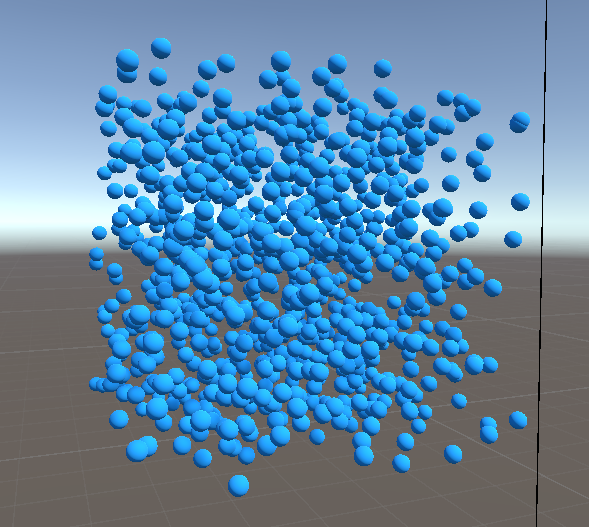
\includegraphics[width=0.5\textwidth]{firstFrameCPU.png}
            \caption{First frame of the simulation using prefabs}
        \end{center}
    \end{figure}

    For convenience, the game object associated with the particle is initially included in the struct for quick position assignment, which may cause performance issues due to high memory usage when the struct is passed frequently in function calls. In the CPU implementation, the highest number of particles tested was 1000.
    
    Next, the particles need to be rendered on to the screen. This is easily done in \textit{Unity} by creating a prefab of the built-in sphere object and instantiating the prefab many times. In order to make the simulation more realistic, a slight variance is added to the particles' starting positions, while maintaining the grid structure. For each instantiation, a particle struct is created and the game object is assigned to it. This struct is then added to a particles array, which contains every particle.

    Once the particles were spawned and bouncing due to gravitational forces, the simulation loop described above was written in \textit{C\#}. See the appendices for methods and calculations. However, the performance and frame rate of the simulation had dropped significantly, to around 2 frames per second.

    \subsubsection{GPU}

    \begin{figure}[H]
        \begin{center}
            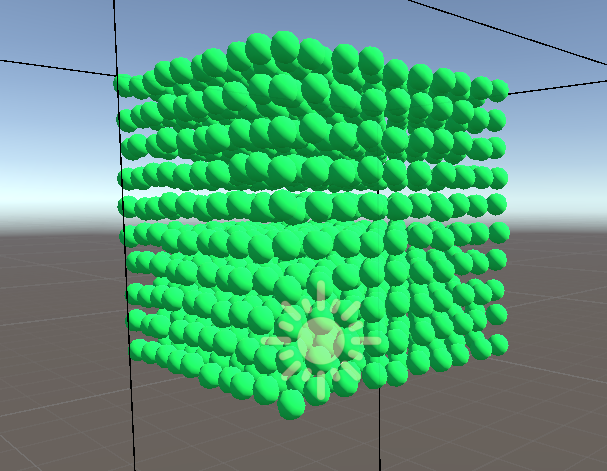
\includegraphics[width=0.5\textwidth]{firstFrameGPU.png}
            \caption{First frame of the simulation using GPU instancing}
        \end{center}
    \end{figure}

    In order to render particles using the GPU, a technique called GPU Instancing is used. This is when all the models are rendered simulataneously with a single draw call. Initially, a surface shader found online was used in this project in order to speed up the process\cite{gpuinstanceshader}. This is eventually rewritten into a vertex and fragment shader that will be explained later in this paper. The rendering logic used is from the same repository. See the appendices for code snippets. Furthermore, another optimisation to note is that the mesh utilised in this method is not the built in sphere object, but rather a low-poly sphere with a lot less triangles, to further enhance performance.

    With this technique, we use a compute shader and HLSL to perform the calculations. We then redraw the particles in their new positions using another single draw call every update frame. For 1000 particles, the same amount of particles as the CPU implementation, this method achieves over 600 frames per second with the same hardware. Furthermore, once we increase the particle count further, performance remains high, maintaining over 500 frames per second for approximately 32,000 particles.

    \subsection{Spatial Hashing}

    The reason the simulation is so slow at this point is because each particle is comparing itself with every other particle in every update step. This is an $O(n^2)$ algorithm and is too slow for large particle counts. The first optimisation involves the aforementioned idea that only the particle's neighbours influence it. The number of calculations performed can thus be considerably reduced with Spatial Hashing.

    Spatial Hashing is a technique that divides a space into a hash table. The table contains hashes that correspond to a small section of the space, a cell, and all the items or particles within that cell\cite{spatialpython}. This reduces the number of calculations as only the cell that the particle is in and its neighbouring cells need to be considered for each particle. 
    
    This algorithm is used at the beginning of each simulation loop. Then, instead of iterating through every particle, each process only needs to check the particles in the neighbour array. There are two slight variants of this method utilised in this project, one for the CPU and one for the GPU.

    \subsubsection{Spatial Hash CPU}

    This section describes the processes involved in the spatial hash used for the \textit{C\#} and CPU implementation. A lot of this method is inspired by a pre-existing implementation found online\cite{sphspatialexample}.

    \begin{algorithm}[H]
        \caption{\textsc{PartialSpatialHashCPU}}
    
        \begin{algorithmic}[1]
            \ForAll{particles $i$}
                \State calculate which cell $i$ is in
                \State find the hash/key for that cell
            \EndFor
            \ForAll{particles $i$}
                \State update the table
            \EndFor
            \ForAll{particles $i$}
                \State find neighbours and store their IDs in $i$.neighbours
            \EndFor
        \end{algorithmic}
    \end{algorithm}

    This method is an improvement as each particle ends up with its own array of neighbours, which is only calculated once at the start of each update loop. The neighbours are stored in a vector within the particle struct and is unique to each particle. This is a huge improvement from before, where each particle calculated its neighbours independently, every update. However, this is at the cost of a lot more storage, as each particle stores their neighbours independently and can introduce repeated data. In regards to performance, the frame rate improves significantly from 2 frames to 15 frames per second on average with 1000 particles still.

    \begin{figure}[H]
        \begin{center}
            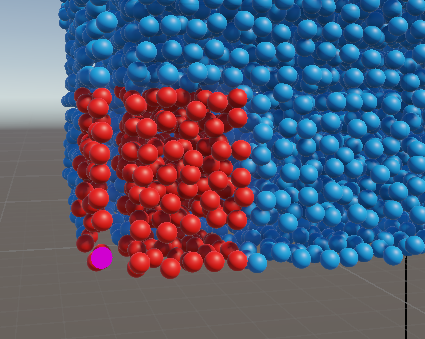
\includegraphics[width=0.5\textwidth]{neighboursCPU.png}
            \caption{Visualisation of neighbour array for pink particle}
        \end{center}
    \end{figure}

    There are still issues with larger particle counts in this implementation due to large memory consumption and the multiple draw calls. In Figure 20, this method was tested with 8000 particles, but the frame rate averaged around 0.5 frames per second. Due to this, the decision was made to move the calculations to the GPU and no further work was completed on this version.

    \subsubsection{Spatial Hash GPU}
    
    The algorithm used for the GPU is more complete. It was a lot easier to debug and improve this version due to the increased performance of the particle rendering. This implementation is created with the aid of multiple online resources\cite{lague}\cite{sphspatialexample}\cite{bitonicyt}\cite{bitonicparallel}.

    \begin{algorithm}
        \caption{SpatialHashGPU}
        \begin{algorithmic}[1]
            \ForAll{particles $i$}
                \State calculate which cell $i$ is in
                \State find the hash key for that cell
            \EndFor
            \ForAll{particles $i$}
                \State sort the particles by hash key
            \EndFor
            \ForAll{particles $i$}
                \State update the lookup table
            \EndFor
        \end{algorithmic}
    \end{algorithm}

    This version differs from the incomplete implementation described above in that it avoids storing a vector of neighbors within each particle structure. Instead, it employs a more efficient approach using a single lookup table. After computing hash keys for all particles, the array of particles is sorted based on these keys. The lookup table then stores the starting index in the sorted array for each unique hash key, allowing for quick access to particles in the same spatial cell. This reduces memory overhead and improves cache coherence. Figure 21 provides a visual explanation of this method created by Sebastial Lague\cite{lague}.
    
    \begin{figure}[H]
        \wideimage[]{spatialHashVisualisation.png}
        \caption{Spatial Hash Visualisation \cite{lague}}
    \end{figure}

    \subsubsection{Cell Calculation}

    The following sections will explain how to implement each step of the algorithm. The code snippets are all in HLSL.

    The space that the particle can occupy (the volume within the bounds of the box) is divided into cells with dimensions equal to a value greater than or equal to the smoothing radius of the particles. This is to guarantee that any neighbouring particles that will provide an influence on this position is either within the same cell or in directly adjacent cells. The simplest way to do this is to divide the current position of the particle by the smoothing radius and return either the floor or ceiling of this - so cells within the same cell have the same cell coordinate.

    \begin{figure}[H]
        \begin{center}
            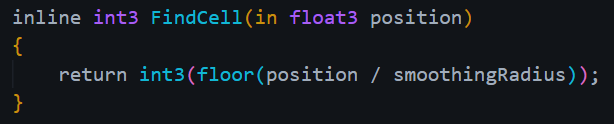
\includegraphics[]{findCell.png}
            \caption{FindCell HLSL}
        \end{center}
    \end{figure}

    \subsubsection{Hash Key Calculation}

    The cell coordinates produced are integer vectors with three entries. This is inefficient for memory and inconvenient for fast lookups; one integer comparison is better than three. In order to convert these vectors into a single integer with minimal overlap, each integer is multiplied by a large hash value and the results are combined using the bitwise XOR operation. Then the hash value is wrapped around the length of the array so that it can be used as an index.

    \begin{figure}[H]
        \begin{center}
            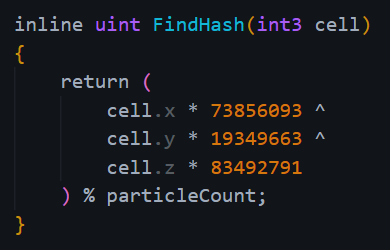
\includegraphics[]{findHash.png}
            \caption{FindHash HLSL}
        \end{center}
    \end{figure}

    \subsubsection{Storing the Hash Keys}

    As these are inline methods, a function that will perform these operations and then store the obtained values in an array needs to be defined. The array begins unsorted with each index being equal to the particle's unique ID. The thread group size attribute is declared at the top of the method. In this implementation, there are 256 threads in each thread group. This means that 256 threads will be launched and use shared resources simulataneously. A power of two is chosen here due to the nature of the sorting algorithm that is used in the next step.

    \begin{figure}[H]
        \begin{center}
            \wideimage[]{hashParticles.png}
            \caption{HashParticles HLSL}
        \end{center}
    \end{figure}

    \subsubsection{Bitonic Sort}
    
    \paragraph{Bitonic Sequence} ``A data-set is bitonic if there exists an index i for which all elements less than or equal to i are in increasing order, and all elements greater than or equal to i are in decreasing order'' \cite{bitonicyt}.

    Something to note is that this definition is valid for sequences that are also entirely increasing or entirely decreasing. As a result, any collection of numbers can be split into a series of bitonic sequences by reducing it down into smaller lists of length 2. This sorting algorithm therefore does not work on lists with a length that is not equal to a power of 2, hence why a thread group of size 256 is used.

    \paragraph{Bitonic Sort} ``A comparison-based sorting algorithm which sorts a data-set by converting the list of numbers into a bitonic sequence. The list is then sorted using a merge function'' \cite{bitonicyt}.

    The pseudocode will be presented below, with the following variables
    \begin{itemize}
        \item arr = the data-set being sorted
        \item lowIndex = the lowest index of the array or sub-array
        \item count = the number of elements in the array or sub-array
        \item direction = whether the bitonic sequence should be increasing or decreasing, 1 = increasing and 0 = decreasing
    \end{itemize}

    \begin{algorithm}
        \caption{BitonicMerge(arr, lowIndex, count, direction)}
        \begin{algorithmic}[1]
            \If {count $>$ 1}
                \State set k = count / 2
                \For {(i = lowIndex; i $<$= lowIndex + k; i++)}
                    \If {direction == (arr[i] $>$ arr[i+k])}
                        \State swap arr[i] and arr[i+k]
                    \EndIf
                \EndFor
                \State \textsc{BitonicMerge}(arr, lowIndex, k, direction)
                \State \textsc{BitonicMerge}(arr, lowIndex + k, k, direction)
            \EndIf
        \end{algorithmic}
    \end{algorithm}

    \begin{algorithm}
        \caption{BitonicSort(arr, lowIndex, count, direction)}
        \begin{algorithmic}[1]
            \If {count $>$ 1}
                \State set k = count / 2
                \State \textsc{BitonicSort}(arr, lowIndex, k, 1)
                \State \textsc{BitonicSort}(arr, lowIndex + k, k, 0)
                \State \textsc{BitonicMerge}(arr, lowIndex, count, direction)
            \EndIf
        \end{algorithmic}
    \end{algorithm}

    The reason that a Bitonic Sort is chosen as our sorting algorithm is because it is a parallel algorithm. This means that multiple operations required in the algorithm can be computed simulataneously. For example, the sequential recusive \textsc{BitonicSort} and \textsc{BitonicMerge} calls do not depend on each other and can therefore be computed in parallel. This is perfect for a GPU based implementation as parallelisation can occur through threading.

    This paper adopts a parallelised version of the Bitonic Sort found in a YouTube tutorial online\cite{bitonicparallel}.

    \begin{figure}[H]
        \begin{center}
            \wideimage[width=\textwidth]{bitonicSortCSharp.png}
            \caption{\textit{C\#} parallelisation}
        \end{center}
    \end{figure}

    \begin{figure}[H]
        \begin{center}
            \wideimage[width=0.9\textwidth]{bitonicSortCompute.png}
            \caption{Bitonic Sort computation HLSL}
        \end{center}
    \end{figure}

    \subsubsection{Update Lookup Table}

    Now that the particles have been sorted according to their hash key values, the lookup table needs to be updated with the changes.

    \begin{figure}[H]
        \begin{center}
            \wideimage[]{updateLookup.png}
            \caption{FillLookupTable HLSL}
        \end{center}
    \end{figure}

    This method iterates through every particle and finds which cell it is in. Then it compares the index of the particle with the starting index currently stored in the table. If this is the first particle in this cell, the value of $\_lookupTable[cellIndex]$ will be an incredibly large number, otherwise it'll be the index of the first particle in that cell. Therefore, when $\textsc{InterlockedMin}(\_lookupTable[cellIndex], id.x)$ is called, if this is the first particle of the cell, its index will be lower than the large default number and will replace this value, otherwise it will remain unchanged.

    \subsubsection{Using the Spatial Hash}

    Once the spatial hash has been implemented, it needs to be integrated into the simulation loop. Note that finding the neighbour-finding logic is moved into the calculation methods.

    \begin{algorithm}[H]
        \caption{Simulation Loop With Spatial Hashing}

        \begin{algorithmic}[1]

            \State reset lookup table

            \ForAll{particles $i$}
                \State calculate the cell and its hash key
            \EndFor

            \State \textsc{SortParticles}()
            
            \ForAll{particles $i$}
                \State update lookup table
            \EndFor

            \ForAll{particles $i$}
                \State calculate density and pressure
            \EndFor

            \ForAll{particles $i$}
                \State compute forces
            \EndFor

            \ForAll{particles $i$}
                \State update velocity and position
                \State resolve collisions
            \EndFor
        \end{algorithmic}

    \end{algorithm}

    By eliminating non-neighboring particles and using a lookup table to store previously computed comparisons, the algorithm's complexity is reduced to $O(n)$ complexity. The worst case scenario is still $O(n^2)$ (if all the particles are within the same cell or neighbouring cells), but this should never be the case due to the forces they exert on each other. 

    With these changes, the simulation achieved frame rates ranging between 250 and 320 for approximately 32,000 particles, a huge improvement to the 15 frames before.

    \subsection{More Forces}

    Two additional forces have not been implemented thus far due to the challenges associated with debugging, stemming from suboptimal optimization. This is no longer an issue thanks to the spatial hash. This section describes their implementations.

    \subsubsection{Surface Tension}

    This section describes an integration of surface tension also given by the aforementioned paper\cite{sca}.

    Molecules in a fluid experience attractive forces from their neighbours. When they are surrounded by neighbours in all directions (when they are not at the surface), these forces are equal in all directions; the net force is \textbf{0}. They are unbalanced at the surface and act in the direction of the surface normal towards the fluid. The effect of this force depends on the two fluids present at the surface (for example water and air), resulting in a tension coefficient $\sigma$.

    To find which particles are on the surface of the fluid, we use the generalised property equation to produce a colour field. The field is 1 in locations a particle is present and 0 otherwise.

    \begin{equation}
        c_S(\textbf{r}) = \sum_{j}{m_j \frac{1}{\rho_j}W(\textbf{r} - \textbf{r}_j, h)}
    \end{equation}

    The smoothing kernel used in these calculations is the previously mentioned Poly6 kernel. The gradient of this colour field is denoted as \textbf{n}, and it represents the surface normal field pointing into the fluid. Its divergence $\nabla \cdot \textbf{n} \equiv \nabla^2 c_S$ measures the curvature of the surface. To obtain these two values, the gradient and Laplacian of the Poly6 kernel are required. Their derivations can be found in the appendices.

    \begin{equation}
        \nabla W_{poly6}(\textbf{r}, h) = \frac{315}{63\pi{h}^9}
        \begin{cases}
            -6(h^2-r^2)^2\textbf{r} & 0 \leq r \leq h \\
            0 & otherwise
        \end{cases}
    \end{equation}

    \begin{equation}
        \nabla^2 W_{poly6}(\textbf{r}, h) = \frac{315}{63\pi{h}^9}
        \begin{cases}
            -6(3h^4 - 10h^2r^2 + 7r^4) & 0 \leq r \leq h \\
            0 & otherwise
        \end{cases}
    \end{equation}
    
    The direction is reversed by taking the negative as the force is trying to flatten the surface.

    \begin{equation}
        \kappa = \frac{-\nabla^2 c_S}{\left|\textbf{n}\right|}
    \end{equation}

    Putting this all together, the following surface force calculation is derived

    \begin{equation}
        \textbf{f}^{surface}_{i} = \sigma \kappa \textbf{n} = -\sigma \nabla^2 c_S(\textbf{r}_i)\frac{\textbf{n}}{\left|\textbf{n}\right|}
    \end{equation}

    There arises a numerical issue when $\left|\textbf{n}\right|$ is too small. To fix this, a threshold is predetermined; the calculations are only considered if this value is greater than the threshold. Similar to the viscosity force, these force calculations can be performed in the same loop as the pressure force.

    \begin{algorithm}[H]
        \caption{\textsc{CalculateForces}(Particle $p$)}

        \begin{algorithmic}[1]
            \State totalPressure $\gets$ [0, 0, 0]
            \State totalViscosity $\gets$ [0, 0, 0]

            \State surfaceForce $\gets$ [0, 0, 0]
            \State colorFieldGradient $\gets$ [0, 0, 0]
            \State coloeFieldLaplacian = 0

            \ForAll{neighbour particles $i$}
                \State offset $\gets$ $p$.position $-\ i$.position
                \State distance $=$ \textsc{magnitude}(offset)

                \If{distance $<$ epsilon}
                    continue
                \EndIf

                \State direction $\gets$ offset $/$ distance
                \State totalPressure $-=$ ($p$.pressure $+\ i$.pressure) $/$ (2 * $i$.density) $*$ \textsc{SpikyGradient}(distance, direction)
                \State totalViscosity += \textsc{ViscosityLaplacian}(distance) *
                \Statex \hspace{\algorithmicindent} ($i$.velocity $-\ p$.velocity) / $i$.density
                \State colorFieldGradient += \textsc{Poly6Gradient}(distance, direction) \Statex \hspace{\algorithmicindent} $/$ $i$.density
                \State colorFieldLaplacian += \textsc{Poly6Laplacian}(distance) $/$ $i$.density
            \EndFor

            \State colorFieldGradient *= particleMass
            \State colorFieldLaplacian *= particleMass

            \State colorFieldGradientLength = \textsc{length}(colorFieldGradient)

            \If {colorFieldGradientLength $>$ threshold}
                \State curvature = -colorFieldLaplacian / colorFieldGradientLength
                \State surfaceForce = -tensionCoefficient * curvature \Statex \hspace{\algorithmicindent} * \textsc{normalize}(colorFieldGradient)
            \EndIf

            \State $p$.force = particleMass * (totalPressure + totalViscosity) + surfaceForce
        \end{algorithmic}

    \end{algorithm}

    \subsubsection{External Forces}

    Although gravity has already been applied, the fluid should be pushed away and interact with objects within the simulation. If the object comes into contact with the particle, it should push the particle in the opposite direction. In this simulation, a single sphere game object was added to the scene; moving it into the box pushes the fluid away. See the appendices for the implementation.

    \subsubsection{Performance}

    These additional calculations have little impact on the overall frame rate of the simulation, it consistently remains within the 250 to 320 frame rate described beforehand for approximately 32,000 particles.

    \subsection{Pre-Computed Constants}

    Another optimisation made at this point involved constants and reducing the overall number of calculations made.

    The first change involes distance checking. Instead of using \textsc(distance)() and comparing this to the smoothing radius, we instead compare the squared distance with the squared smoothing radius, only square rooting when needed. This is because calculating the square root is a very expensive computation and should only be done when needed. This can also be extended by precomputing the squared smoothing radius and storing it in a variable, as this is a value that will not change during runtime.

    There are other constants that can be precomputed also. For example, each smoothing kernel involves multiplication of a fraction that depends on $h$, the smoothing radius. As $h$ is a constant, these can also be calculated and passed to the compute shader once, as shown below.

    \begin{figure}[H]
        \begin{center}
            \wideimage[width=1.1\textwidth]{precomputeMults.png}
            \caption{Precomputed Variables \cite{lague2}}
        \end{center}
    \end{figure}

    This improvement increased the consistency of the frame rate; it remains within 280 to 340 frames per second.

    \subsection{Circles}

    It was at this point that the rendering shader was rewritten. Thanks to the \textit{OpenGL} learned at the beginning, it was possible to rewrite the Surface shader into a Vertex and Fragment shader. See the appendices for the new shader code. The reason for for this was to change the mesh that was being rendered. 
    
    Previously, a low-poly sphere was being used, consisting of 60 triangles. Instead of a 3D mesh, a quad may be utilised instead, which consists of only 2 triangles. In order to maintain the 3D appearance, the vertex shader was rewritten to ensure that the meshes were constantly facing the camera. This was done using a tutorial found online\cite{lague2}.

    The snippet below positions a quad in world space and orients it to always face the camera by performing the following steps:
    \begin{itemize}
        \item Start with the quad's world position as the centre
        \item Scale the vertex coordinates to determine visual dimensions
        \item Extract the camera's right and up directions; the x and y axes in world space
        \item Offset the quad's vertices using these vectors, making sure the quad remains perpendicular to the camera's forward direction
    \end{itemize}

    \begin{figure}[H]
        \begin{center}
            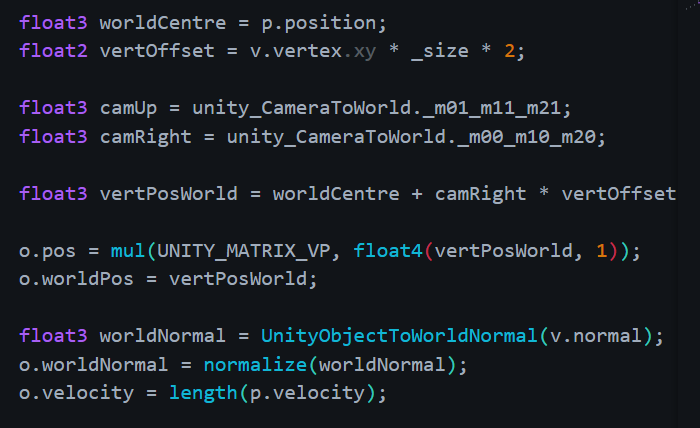
\includegraphics[]{cameraLogic.png}
            \caption{Camera Logic Vertex Shader \cite{lague2}}
        \end{center}
    \end{figure}

    In order to maintain a spherical appearance, the corners of the quad need to be discarded. This is done by the Fragment Shader:
    
    \begin{itemize}
        \item Shift the UV coordinates so that the quad's centre is (0,0)
        \item Scale the coordinates to range between -1 and 1
        \item Compute the squared distance from the centre using the dot product $x^2 + y^2$
        \item Discards the fragment if this value is greater than 1 (the circle's radius)
    \end{itemize}

    \begin{figure}[H]
        \begin{center}
            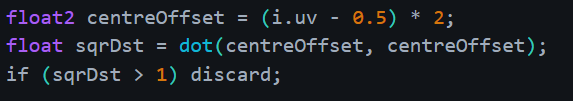
\includegraphics[]{circleLogic.png}
            \caption{Circle Logic Fragment Shader \cite{lague2}}
        \end{center}
    \end{figure}

    For any fragments not discarded, the colour of the circle is set based on the particle's velocity. A rainbow gradient was chosen for the purposes of the demonstration but is easily adjustable due to the formula used\cite{colours}.

    \begin{figure}[H]
        \begin{center}
            \wideimage[]{paletteHelper.png}
            \caption{Colour Palette Formula \cite{colours}}
        \end{center}
    \end{figure}

    The rainbow gradient is achieved with the following values:
    \begin{itemize}
        \item a = $(0.50, 0.50, 0.50)$
        \item b = $(0.50, 0.50, 0.50)$
        \item c = $(1.00, 1.00, 1.00)$
        \item d = $(0.00, 0.33, 0.67)$
    \end{itemize}

    \begin{figure}[H]
        \begin{center}
            \wideimage[width=0.5\textwidth]{finalAppearance.png}
            \caption{Rainbow gradient and circle particles}
        \end{center}
    \end{figure}

    With this optimisation, the simulation's frame rate improved from 340 frames to around 400 frames with approximately 40,000 particles. This was the final product of this dissertation.

    \newpage

    \section{Results and Evaluation}
    \label{sec:resultsandevaluation}

    This project produced three simulations with varying levels of completion, illustrating the iterative nature of the Agile development process.

    \subsection{Agile Development}

    One of the key strengths of employing the Agile methodology in this project was the flexibility it offered in adapting to the strict time frame presented. The iterative nature allowed quick changing of software and tools, without the constaints of a more rigid development plan. This was especially helpful when the decision to swap over completely from \textit{OpenGL} to \textit{Unity} was made; there was no pause or replanning required. Furthermore, this allowed for a more self-directed workflow, due to independent development and research. However, there was still access to a supervisor if required. Overall, there was a more efficient and responsive development process due to the balance between independence and guidance provided.

    Despite these advantages, there were also a few issues with this method. Due to the encouraged autonomy, too much independence led to lacking time structure, especially in the absence of external accountability. Supervisor support should have been utilised more than it was. Additionally, progress could have definitely been documented or recorded better; some \textit{Git} commits contained a large number of changes, which made it difficult to track specific modifications and the affect on the frame rate as a result of them.

    Overall, Agile development provided significant contributions to the adaptability and progress of the project. While it was suited for dynamic and evolving projects such as this one, the methodology was very dependent on the discipline of the people utilising it.

    \subsection{OpenGL Simulation}

    One of the ``simulations" produced in this dissertation was the previously mentioned grid of cubes developed using \textit{C++} and \textit{OpenGL}. Due to the lack of features and the use of shaders and GPU-based rendering, the simulation achieved a consistently high frame rate. However, it did not portray realistic fluid behaviour, as the particles were only influenced by a gravitational force and experienced no inter-particle interactions (they passed through each other in straight lines with minimal collision detection at a boundary).

    Although this method was ultimately abandoned, it still proved to be very beneficial from a learning perspective. A lot of the overall technical knowledge gained from this project was from the initial research required to use the \textit{OpenGL} graphics API. Hands-on experience with the graphics rendering pipeline through the use of \textit{OpenGL} and custom shaders provided key insights into low-level rendering processes and enabled improvements in the \textit{Unity} implementation. For example, the rendering shader was rewritten independently with this acquired knowledge. Furthermore, the process of learning compute shaders was greatly simplified and sped up the development process of this simulation significantly. Overall, it was a very important part of this project as acquiring low-level graphics programming skills improved technical confidence and enabled both this project and future projects.

    In hindsight, while appreciative of the knowledge gained from this implementation, if supervisor support were further utilised, the decision to swap software could have been made a lot earlier. Due to the significant portion of development time occupied, there was a lot less time allocated to the final implementation as a whole. More time could have been allocated to optimisation techniques if the simulation's physics were completed at an earlier stage. Learning to balance exploration and knowledge with results is an important skill to improve in the future.

    \subsection{Unity CPU Simulation}

    The next simulation produced in this project was a CPU-based implementation with \textit{C\#} and \textit{Unity}. This achieved the same things that the previous simulation did, a grid of particles that moved due to gravitational forces, but had a lower frame rate, starting at around 300 frames per second for 1000 particles. This is not a large particle count, but larger numbers decreased this value quite significantly, so this was the initial count chosen. After the physics was implemented, the performance had dropped, peaking at 2 frames per second. With the first optimisation technique, spatial hashing, this was improved by over 20 times, achieving a consistent frame rate of over 15 frames per second for 1000 particles. However, this was nowhere near the desired number of particles, and increasing the count still produced detrimental performance reduction. Thus, the next optimisation was to switch to a GPU-based implementation.

    An advantage of this CPU implementation was prior experience with \textit{Unity} from a full \textit{C\#}-based perspective. This reduced the learning curve significantly and thus greatly reduced the amount of time required to reach this point in development. Due to the familiarity of the environment, faster and more confident prototyping was possible. Moreover, confidence in the programming language facilitated the process of translating the academic papers used, from physics equations into executable code. Concepts such as Object-Oriented Programming and Unity's Monobehavior scripts were already well understood, further enhancing efficiency and accuracy within the implementation. As a result, a focus on particle behaviour and performance optimisation was possible.

    There were unfortunately still a number of issues with this implementation. There was a lot of problems with memory, as the algorithm developed involved passing through entire structs between functions, causing repeated data to be recreated as copies, leading to significant performance overhead. Furthermore, this repeated copying was not cache-friendly, leading to slower data access. An improvement on this would have been to either pass the information to the methods by reference, or to rewrite the logic in a way that did not involve entire particle structs being passed through every step of the algorithm. Such a small particle count producing a low frame rate caused the debugging process to be quite frustrating, due to the difficulty of efficiently testing changes, hindering the ability to identify bottlenecks within the code logic. 
    
    There were a lot more optimisations that could have been implemented to improve these issues. For example, multithreading is supported in \textit{C\#}. However, the CPU has significantly less threads than the GPU and is not as good at performing calculations quickly. As a result, it was deemed unnecessary to implement threading on this version of the project; it was more time efficient to move on to the GPU implementation immediately.

    The combination of these issues and the limited time frame contributed to the decision of abandoning this second implementation and continuing to a fully GPU-based implementation within Unity, though the initial programming required to produce this was beneficial in simplifying and speeding up the GPU implementation process.


    \subsection{Unity GPU Simulation}
    
    The final simulation produced in this project was a GPU-based implementation with \textit{HLSL} and Compute Shaders with \textit{Unity}. When this version reached the same development point as the OpenGL implementation - a grid of particles affected by gravitational forces - it also achieved very high frame rates, averaging around 600 frames per second for 1,000 particles. When the physics was initially applied with no optimisations, the frame rate decreased to around 300 frames per second for 1,000 particles and less than 100 for 32,000 particles. Integrating the spatial hash algorithm into this simulation improved the average frame rate, achieving results between 250 to 320 frames per second for 32,000 particles. Manually precomputing and setting constant values into the simulation further improved the frame rate, to around 280-340 frames per second due to the significant reduction in the number of calculations performed. Finally, making the particles 2D circles that maintain their 3D appearance improved the overall frame rate even further to around 400 frames for 32,000 particles.
    
    However, at this point when testing the impact of higher particle counts, there was an issue noticed regarding the box bounds that the particles were contained in. In the first frame, the particles were not forming a full grid as the grid was too large for the box bounds. This may have caused issues in the first few frames of the simulation but the particles quickly rectified this error and returned to a stable fluid flow.

    \begin{figure}[H]
        \begin{center}
            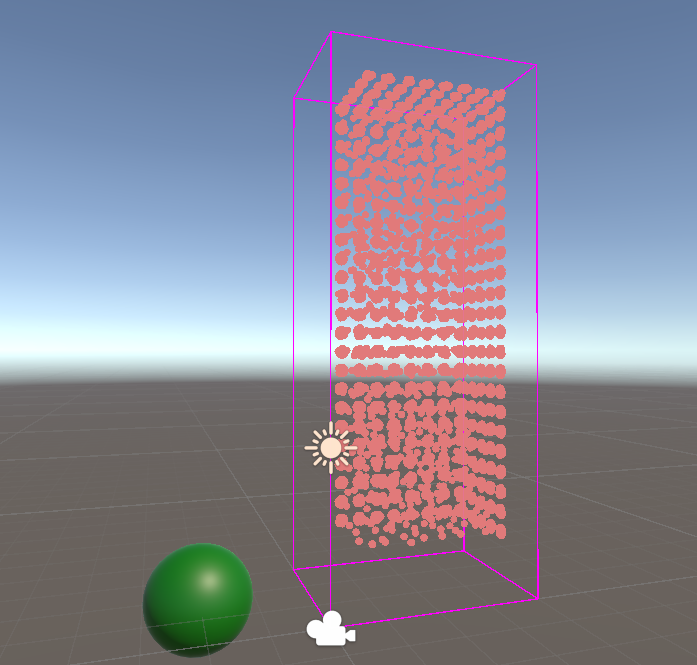
\includegraphics[width=0.6\textwidth]{firstFrameSmallBox.png}
            \caption{First Frame Small Box}
        \end{center}
    \end{figure}
    
    When the box bound was increased before running the simulation, the frame rate consistently remained in the 600s. The underlying reasoning is uncertain, but it is believed that it may be due to the collision resolution calculations. This was noticed too late in the development stage and further investigation could not be performed. The remaining results for this simulation will however involve box dimensions that satisfy the entire grid formation.

    \begin{figure}[H]
        \begin{center}
            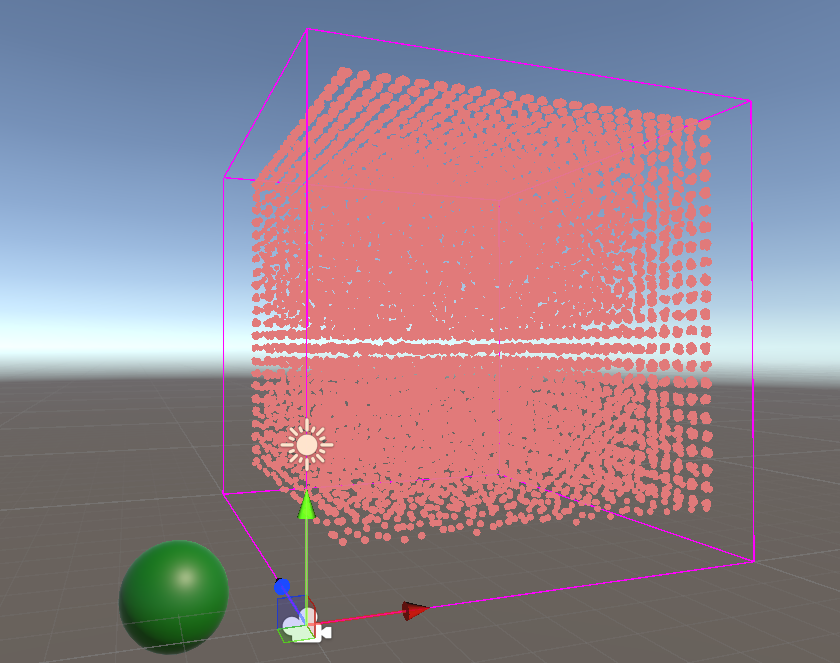
\includegraphics[width=0.75\textwidth]{firstFrameBigBox.png}
            \caption{First Frame Big Box}
        \end{center}
    \end{figure}

    \begin{figure}[H]
        \begin{center}
            \wideimage[width=1.15\textwidth]{exponentialRegression.png}
            \caption{Particle Count vs. Frame Rate \cite{desmos}}
        \end{center}
    \end{figure}

    Figure 35 shows the frame rates obtained for different particle counts. This graph was created using Desmos, an online graphing calculator\cite{desmos}. There appears to be an exponential relationship between frame rate and particle count for this simulation. In the case of a video game, 60 frames per second is usually the target to maintain a smooth gameplay experience, and this simulation achieves a remarkable count of over 390,000 particles at this FPS. 
    
    A slight error noticed when testing larger particle counts was that some particles remained in the grid structure for a longer time than anticipated.

    \begin{figure}[H]
        \begin{center}
            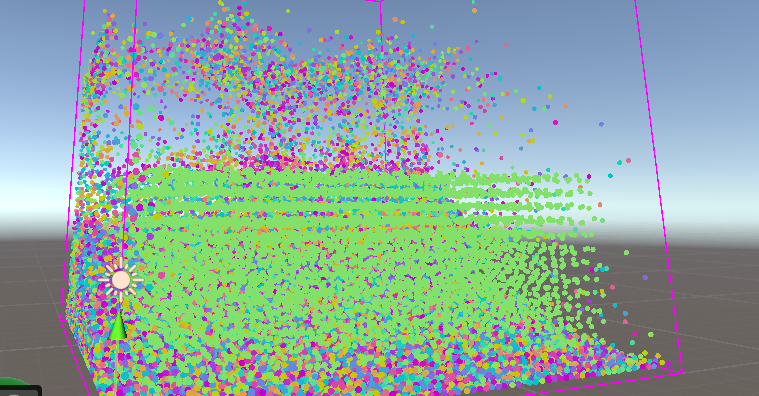
\includegraphics[]{gridIssues.png}
            \caption{Grid Simulation Issues}
        \end{center}
    \end{figure}

    There has not been a fix implemented and therefore, although this issue is eventually resolved automatically, it is not recommended to use this simulation for larger particle counts.

    This simulation offers several improvements over the previous two versions. Most notably, it is more complete and can handle more than 1,000 particles. This significant improvement in performance is partly due to the improved memory management; it does not copy structs across methods and involves multi-threading, unlike the CPU implementation. This change also allows it to handle substantially greater particle counts with little trouble.

    This simulation does suffer from a few issues. At the moment, it is just a demonstration of fluid physics. More code is required to make the fluid fully interactable; it is currently only affected by the sphere within the scene. Furthermore, it is not currently possible to create two different fluids simulataneously without writing more code. There is also the aforementioned issue with the reduced frame rate issues when the grid does not fit fully inside the initial box, and the delay in particle movement for larger particle counts. This heavily affects its scalability and needs further work to improve. Finally, it still looks like a collection of particles rather than a full body of liquid. Although this was out of the scope of this project, there is definitely more work that could be done in this area.

    Overall, this is a satisfying result for an initial project in the area of fluid simulation. Achieving a fluid flow that exhibits a high degree of realism is a gratifying outcome.

    \subsection{Requirements}

    Functional requirements 1-5 were satisfied: the fluid simulation is rendered with particles that represent parcels of fluid - this is the SPH approach that was consistently used throughout the paper. The calculations involve consider the fluid's viscosity, density and pressure, satisfying functional requirement 2. It is also affected by the position of the sphere object within the scene and by gravitational forces, satisfying functional requirements 3 and 5. Finally, the fluid does not leave the assigned box dimensions, and are affected by the box changing dimensions. This satisfies the final functional requirement, number 4.

    Non-functional requirements 1, 2, 5 and 6 were satisfied: the simulation achieves an average frame rate of 600 for over 32,000 particles, and maintains over 60 frames for up to 390,000 particles, satisfying non-functional requirement 1. Evidence of memory reductions are described through the lookup table improvment in the spatial hashing algoritm and the struct-copying issues mentioned in the CPU implementation. This satifies non-functional requirement 2. The properties of the fluid can be adjusted in the Unity inspector in real time, and the fluid reacts to these changes with no delay. This satisfies non-functional requirement 5. Although more code is required to implement new fluid types, the simple adjustability of the fluid properties mentioned earlier will make future implementation of other fluids easier. This satisfies non-functional requirement 6.

    When the box dimensions are changed, the program does sometimes stutter slightly. This does not satisfy non-functional requirement 4. The aforementioned issue with large particle count grids dissatisfies non-functional requirement 3. These issues could not be rectified in the given time frame, but are possible in future work.

    \newpage

    \section{Conclusion}
    \label{sec:conclusion}
    \subsection{Aims and Objectives}
    \subsection{What Was Learned}
    \subsection{Future Work}

    \newpage

    \section{References}
    \label{sec:references}
    \bibliography{references}

    \newpage

    \section{Appendices}
    \label{sec:appendices}

    \subsection{Unity Asset Store}

    \begin{figure}[H]
        \wideimage[]{unityStore1.png}
        \caption{Most popular results for "fluid simulation" \cite{unityasset}}
    \end{figure}

    \begin{figure}[H]
        \wideimage[]{unityStore2.png}
        \caption{Cheapest results for "fluid simulation" \cite{unityasset}}
    \end{figure}

    \begin{figure}[H]
        \wideimage[]{stylizedWaterURP.png}
        \caption{Example of surface-only Unity asset \cite{stylized}}
    \end{figure}

    \subsection{Learn OpenGL and graphics}

    \subsection{Kernel Derivations}

    \subsubsection{Spiky Kernel Gradient}

    \begin{proof}
        Spherical Gradient is defined as

        $$\nabla f = \frac{\partial{f}}{\partial{r}}\textbf{e}_r + \frac{1}{r}\frac{\partial{f}}{\partial{\theta}}\textbf{e}_{\theta} + \frac{1}{r \sin{\theta}}\frac{\partial{f}}{\partial{\phi}}\textbf{e}_{\phi}$$
        
        where $\textbf{e}_{r}, \textbf{e}_{\theta}, \textbf{e}_{\phi}$ are the unit direction vectors in the radial, polar and azimuthal directions respectively.

        Due to the radial symmetry of smoothing kernels, this is simplified to

        $$\nabla f = \frac{\partial{f}}{\partial{r}}\textbf{e}_r$$

        $$\nabla W_{spiky}(\textbf{r}, h) = \frac{\partial{W}}{\partial{r}} \cdot \frac{\textbf{r}}{r}$$

        $$\frac{\partial{W}}{\partial{r}} = \frac{15}{\pi{h}^6} \cdot \frac{\partial}{\partial{r}} (h - r)^3$$

        Applying the chain rule

        $$\frac{\partial}{\partial{r}} (h - r)^3 = 3 \cdot (h - r)^2 \cdot (-1) = -3(h - r)^2$$

        Therefore

        $$\nabla{W_{spiky}(\textbf{r}, h)} = \frac{15}{\pi{h}^6} \cdot -3(h - r)^2 \cdot \frac{\textbf{r}}{r} = \frac{-45}{\pi{h}^6}\begin{cases}
            (h - r)^2 \cdot \frac{\textbf{r}}{r} & 0 \leq r \leq h \\
            0 & otherwise
        \end{cases}$$
    \end{proof}

    \subsubsection{Poly6 Gradient}

    \begin{proof}
        Using the spherical gradient from $7.3.1$

        $$\nabla W_{poly6}(r, h) = \frac{\partial{W}}{\partial{r}} \cdot \frac{\textbf{r}}{r}$$

        $$\frac{\partial{W}}{\partial{r}} = \frac{315}{64\pi{h}^9} \cdot \frac{\partial}{\partial{r}} (h^2 - r^2)^3$$

        Applying the chain rule

        $$\frac{\partial}{\partial{r}} (h^2 - r^2)^3 = 3 \cdot (h^2 - r^2)^2 \cdot (-2r) = 6r(h^2 - r^2)^2$$

        Therefore

        \begin{align*}
            \nabla W_{poly6}(\mathbf{r}, h) 
            &= \frac{315}{64\pi h^9} \cdot 6(h^2 - r^2)^2 \cdot r \cdot \frac{\mathbf{r}}{r} \\
            &= \frac{315}{64\pi h^9}
            \begin{cases}
                6(h^2 - r^2)^2 \cdot \textbf{r} & 0 \leq r \leq h \\
                0 & otherwise
            \end{cases}
        \end{align*}
    \end{proof}

    \subsubsection{Poly6 Laplacian}

    \begin{proof}
        Spherical Laplacian is defined as

        $$\nabla^2 f = \frac{1}{r^2}\frac{\partial}{\partial{r}}\left(r^2\frac{\partial{f}}{\partial{r}}\right) + \frac{1}{r^2\sin\theta}\frac{\partial}{\partial{\theta}}\left(\sin\theta\frac{\partial{f}}{\partial{\theta}}\right) + \frac{1}{r^2\sin^2\theta}\left(\frac{\partial^2{f}}{\partial{\phi^2}}\right)$$

        Due to the radial symmetry of the kernel functions, this is simplified to

        $$\nabla^2 f = \frac{1}{r^2}\frac{\partial}{\partial{r}}\left(r^2\frac{\partial{f}}{\partial{r}}\right)$$
        
        Using the chain rule

        $$\frac{\partial}{\partial{r}}\left(r^2\frac{\partial{f}}{\partial{r}}\right) = 2r \cdot \frac{\partial{f}}{\partial{r}} + r^2 \cdot \frac{\partial^2{f}}{\partial{r^2}}$$

        $$\frac{1}{r^2} \left(2r \cdot \frac{\partial{f}}{\partial{r}} + r^2 \cdot \frac{\partial^2{f}}{\partial{r^2}}\right) = \frac{2}{r} \cdot \frac{\partial{f}}{\partial{r}} + \frac{\partial^2{f}}{\partial{r^2}}$$

        Therefore

        $$\nabla^2 W(\textbf{r}, h) = {2}{r} \cdot \frac{\partial{f}}{\partial{r}} + \frac{\partial^2{f}}{\partial{r^2}}$$

        Using the result from $7.3.2$, let $C = \frac{315}{64\pi{h}^9}$

        \begin{align*}
            \frac{\partial W^2}{\partial r^2} 
            &= \frac{\partial}{\partial r} \left(-6C(h^2 - r^2)^2 r\right) \\
            &= -6C \cdot \frac{\partial}{\partial r} \left[(h^2 - r^2)^2 \cdot r\right] \\
            &= -6C \cdot \left[(h^2 - r^2)^2 \cdot \frac{d}{dr}(r) + r \cdot \frac{d}{dr}(h^2 - r^2)^2\right] \\
            &= -6C \cdot \left[(h^2 - r^2)^2 \cdot 1 + r \cdot 2(h^2 - r^2) \cdot (-2r)\right] \\
            &= -6C \cdot \left[(h^2 - r^2)^2 - 4r^2(h^2 - r^2)\right] \\
            &= -6C \cdot (h^2 - r^2) \cdot \left[(h^2 - r^2) - 4r^2\right]
        \end{align*}

        Combining these results

        \begin{align*}
            \frac{2}{r} \cdot \frac{\partial f}{\partial r} + \frac{\partial^2 f}{\partial r^2}
            &= \frac{2}{r} \cdot \left(-6Cr(h^2 - r^2)^2\right) + \left(-6C \cdot (h^2 - r^2)\left[(h^2 - r^2) - 4r^2\right]\right) \\
            &= -12C \cdot (h^2 - r^2)^2 -6C \cdot (h^2 - r^2) \cdot \left[(h^2 - r^2) - 4r^2\right] \\
            &= -6C \cdot (h^2 - r^2) \left[2(h^2 - r^2) + (h^2 - r^2 - 4r^2)\right] \\
            &= -6C \cdot (h^2 - r^2) \left[3(h^2 - r^2) - 4r^2\right] \\
            &= -6C \cdot (h^2 - r^2) \cdot (3h^2 - 7r^2) \\
            &= -6C \cdot (3h^4 - 10h^2r^2 + 7r^4) \\
            &= C \cdot \left[-6(3h^4 - 10h^2r^2 + 7r^4)\right]
        \end{align*}

        Therefore

        $$\nabla^2 W(\textbf{r}, h) = \frac{315}{64\pi{h}^9}
        \begin{cases}
            -6(3h^4 - 10h^2r^2 + 7r^4) & 0 \leq r \leq h \\
            0 & otherwise
        \end{cases}$$
    \end{proof}
\end{document}